%%%%%%%%%%%%%%%%%%%%%%%%%%%%%%%%%%%%%%%%%
% Short Sectioned Assignment
% LaTeX Template
% Version 1.0 (5/5/12)
%
% This template has been downloaded from:
% http://www.LaTeXTemplates.com
%
% Original author:
% Frits Wenneker (http://www.howtotex.com)
%
% License:
% CC BY-NC-SA 3.0 (http://creativecommons.org/licenses/by-nc-sa/3.0/)
%
%%%%%%%%%%%%%%%%%%%%%%%%%%%%%%%%%%%%%%%%%

%----------------------------------------------------------------------------------------
%	PACKAGES AND OTHER DOCUMENT CONFIGURATIONS
%----------------------------------------------------------------------------------------

\documentclass[titlepage, paper=a4, fontsize=11pt]{scrartcl} % A4 paper and 11pt font size

\usepackage[T1]{fontenc} % Use 8-bit encoding that has 256 glyphs
\usepackage{fourier} % Use the Adobe Utopia font for the document - comment this line to return to the LaTeX default
\usepackage[english]{babel} % English language/hyphenation
\usepackage{amsmath,amsfonts,amsthm} % Math packages
\usepackage{listings}
\usepackage{graphicx}

\usepackage{lipsum} % Used for inserting dummy 'Lorem ipsum' text into the template


\usepackage{sectsty} % Allows customizing section commands
\allsectionsfont{\centering \normalfont\scshape} % Make all sections centered, the default font and small caps

\usepackage{fancyhdr} % Custom headers and footers
\pagestyle{fancyplain} % Makes all pages in the document conform to the custom headers and footers
\fancyhead{} % No page header - if you want one, create it in the same way as the footers below
\fancyfoot[L]{} % Empty left footer
\fancyfoot[C]{} % Empty center footer
\fancyfoot[R]{\thepage} % Page numbering for right footer
\renewcommand{\headrulewidth}{0pt} % Remove header underlines
\renewcommand{\footrulewidth}{0pt} % Remove footer underlines
\setlength{\headheight}{13.6pt} % Customize the height of the header

\numberwithin{equation}{section} % Number equations within sections (i.e. 1.1, 1.2, 2.1, 2.2 instead of 1, 2, 3, 4)
\numberwithin{figure}{section} % Number figures within sections (i.e. 1.1, 1.2, 2.1, 2.2 instead of 1, 2, 3, 4)
\numberwithin{table}{section} % Number tables within sections (i.e. 1.1, 1.2, 2.1, 2.2 instead of 1, 2, 3, 4)

\setlength\parindent{0pt} % Removes all indentation from paragraphs - comment this line for an assignment with lots of text
\numberwithin{figure}{section}
\renewcommand{\thefigure}{\arabic{figure}}

%----------------------------------------------------------------------------------------
%	TITLE SECTION
%----------------------------------------------------------------------------------------

\newcommand{\horrule}[1]{\rule{\linewidth}{#1}} % Create horizontal rule command with 1 argument of height

\title{	
\normalfont \normalsize 
\textsc{University of Virginia} \\ [25pt] % Your university, school and/or department name(s)
\horrule{0.5pt} \\[0.4cm] % Thin top horizontal rule
\huge CS 6161 Algorithms \\
\huge Problem Set 5 \\ % The assignment title
\horrule{2pt} \\[0.5cm] % Thick bottom horizontal rule
}

\author{Shawn (Shuoshuo) Chen\\sc7cq@virginia.edu\\Group partner: Rolph Recto\\ rjr7je@virginia.edu}

\date{\normalsize\today} % Today's date or a custom date

\begin{document}

\maketitle % Print the title

%----------------------------------------------------------------------------------------
%	PROBLEM 1
%----------------------------------------------------------------------------------------

\section*{Problem 1}
First, we show that given an algorithm that solves HP, the st-HP can also be solved within an extra polynomial time overhead. For a given graph, assume there is an oracle that gives the yes/no answer to the HP problem in constant time. We can thus construct an algorithm that solves st-HP given a specified pair of start/end points $(s,t)$. We can attach a point $u$ to $s$ with only one edge from $u$ to $s$, and similarly attach $v$ to $t$ with only one edge from $v$ to $t$. We call this new graph including $u,v$ as $G'$. Once we have $G'$, we can call the solver for HP with input $G'$. If the oracle says yes for $G'$, then we know $(s,t)$ must be the end points for $G$ because $(u,v)$ can only be reachable via $s,t$. Otherwise, if the oracle says no, that means even there exists a HP, $(s,t)$ are not the end points, which is not we are looking for. Since attaching two points to $G$ can be done in constant time, the overhead is obviously polynomial. \\

Next, we show that given an algorithm that solves st-HP, the st-S-HP can also be solved within an extra polynomial tme overhead. Since we are already able to solve the st-HP problem, we can recursively find out the path given $(s,t)$. After being confirmed with a yes by the oracle (meaning the HP exists), we remove $(s,t)$ from the graph and thus get a new graph $G^*$. We randomly pick two points $(s^*,t^*) \in V-2$ as the new end points. Then, invoke the st-HP solver again with input $(G^*,s^*,t^*)$. If the oracle says yes, remove $(s^*,t^*)$ and pick two new random points $(s^{**},t^{**}) \in V-4$ and repeat the process again. Otherwise, if the oracle says no, pick another pair of points from $V-2$ and do it again. Eventually, if a HP does exist, we will end up using up all the points and the last call to the solver will just be two points connected by an edge. So after this recursive process, we can get a chain of end points, which is the HP we are looking for. Note that the worst case we could run into is to call the st-HP solver $O(n^2)$ times and get a yes from the last call. And then we go into a nested subgraph and recursively call the st-HP $O(n)$ times until we have a definite path. Overall, this algorithm runs in at most $O(n^3)$ time. \\

Finally, we show that given an algorithm that solves st-S-HP, the S-HP can also be solved within an extra polynomial time overhead. We can start by calling the solver for HP to see if there exists a valid HP. Here we assume there exists such an HP. We now know the solver for st-S-HP returns either a no or an HP for the input implying a yes. Thus, to solve the generic case of S-HP, we can randomly pick two points from $G=(V,E)$ as the end points. Then, call the solver for st-S-HP. If the returning answer is an HP, then we are done. But if it returns a no, we need to choose another pair of end points and call the solver again until we get the HP. It is easy to see that in the worst case, we have to call the subroutine $O(n^2)$ times by covering all possible pairs of end points. So this algorithm runs in polynomial time. \\

To sum up the above, we can solve S-HP by calling the solver for HP within a polynomial time overhead. Thus, we have reduced S-HP to HP.



%----------------------------------------------------------------------------------------
%	PROBLEM 2
%----------------------------------------------------------------------------------------

\section*{Problem 2}
First, we prove (a) graph G is connected if it has n-1 edges and no cycle. \\
Assume there are k connected subgraphs in G. By the definition of tree, an undirected, connected, acyclic graph is a tree. Thus the k subgraphs are k trees. Thus, each subgraph has $|V_i|-1$ edges, which will be proved later. Then sum up all the edges in these k subgraphs, we get $|V|-k = n-k$ edges. According to property (b), there must be $k=1$, which effectively makes G connected as a whole component. \\

Next, we prove (b) graph G has n-1 edges if it is connected and acyclic. \\
We can prove it by showing $|E| \geq |V| -1$ and $|E| \leq |V| -1$. \\
By induction, if $|V|=1,2$, $|E| \geq 0,1$ is trivially true. Then assume it is also true for $|V| \leq n$. For a graph with $n+1$ vertices, choose a random vertex $v$, remove $v$ and its incident edges. Then the graph is divided into $k$ connected subgraphs with $n_1, n_2, ... , n_k$ vertices respectively. By assumption, there is $\sum_1^k |E_i| \geq \sum_1^k (n_i -1)=\sum_1^k n_i - k = n-k$. Now add $v$ back to G, since G is connected, there should be at least one edge between $v$ and each subgraph. Therefore,
$|E| \geq \sum_i^k |E_i| + k = n-k+k = n = |V| - 1$. \\
Similarly, it is trivial that a connected graph with 1 or 2 vertices has 0 or 1 edge. Assume $|E| \leq |V| -1$ for $|V| \leq n$. Removing an arbitary edge from G separates the graph into $k \geq 2$ connected subgraphs. Each subgraph, by definition, is a tree. Because each subgraph has less than $|V|=n$ vertices, it satisfies $|E_i| \leq |V_i| - 1$. Sum up all edges in all subgraphs, there is $\sum_1^k |E_i| \leq |V| - k \leq |V| - 2$. After adding the removed edge back, we have $|E| \leq |V| - 1$. \\
Therefore, we conclude $|E| = |V| - 1 = n-1$. \\

Finally, we prove (c) graph G has no cycle if it is connected and it has n-1 edges. \\
Suppose there is a cycle in G containing k vertices: $v_1, v_2, ... , v_k$. Let $G_k = (V_k, E_k)$ be the subgraph consisting of the cycle. Then there is $|V_k| = |E_k| = k$. If $k \textless |V|$, there must exist a vertex $v_{k+1} \in V - V_k$ that is adjacent to $v_i \in V_k$ due to G is connected. Let $G_{k+1} = (V_{k+1}, E_{k+1})$ be the subgraph with $V_{k+1} = V_k \cup \{v_{k+1}\}$ and $E_{k+1} = E_k \cup \{(v_i, v_{k+1})\}$. Note there is $|V_{k+1}| = |E_{k+1}| = k$. If $k+1 \textless |V|$, we can continue to $G_{k+2}$ until it reaches $G_n$ where $n=|V|, V_n=V, |E_n|=|V_n|=|V|$. Since $G_n$ is a subgraph of G, there is $|E| \geq |V|$. It contradicts the property that $|E|=|V|-1=n-1$. \\




%----------------------------------------------------------------------------------------
%	PROBLEM 3
%----------------------------------------------------------------------------------------

\section*{Problem 3}
Prim's algorithm can be implemented as follows: \\
For a weighted, undirected graph G = (V, E), \\
1. Pick a random $v \in V$ and let the vertices set of the MST $S=\{v\}$. \\
2. Let the MST $T=\emptyset$. \\
3. While $S \neq V$: \\
---- 3a. Choose a least-cost edge $e=(u,v)$ such that $u \in S, v \in (V-S)$. \\
---- 3b. Add $e=(u,v)$ to $T$. \\
---- 3c. Add $v$ to $S$. \\

As above shows, the algorithm needs to visit all the incident vertices for a vertex in $S$, which could be $|V|$ vertices in the worst case. And it needs to iterate over all vertices in $S$ to find the minimum weighted edge, where $|S| \leq |V|$. Therefore, this algorithm can run with time complexity at most $O(|V|^2)$. \\

Now we need to prove the correctness of Prim's algorithm. This would be done in two parts: (1) Prim's algorithm produces a spanning tree. (2) Prim's algorithm correctly finds an MST. \\

For (1): At every iteration of Prim's algorithm, there must be an edge found that connects a vertex in $S$ to another vertex in $V-S$. Since $G$ itself is connected, there always exists a path to every vertex. And $T$ exists as a tree in $S$. The output of Prim's algorithm thus should be a tree because the vertices added to $S$ are connected and adding connected vertices to a tree still forms a tree. \\

For (2): Let $T$ be the spanning tree produced by Prim's algorithm and $T^*$ be any MST in $G$. We need to prove $c(T)=c(T^*)$ so that T is MST. \\
If $T=T^*$, it is trivial to see that $c(T)=c(T^*)$. \\
Otherwise $T \neq T^*$, there is $T-T^* \neq \emptyset$. Let $e=(u,v)$ be any edge in $T-T^*$. When
$e$ is added to $T$, it must be a least-cost edge crossing some cut $(S, V-S)$. Since $T^*$ is MST, there should also be a path from $u$ to $v$ in $T^*$, which implies there exists a $e'=(x,y)$ crossing the same cut $(S, V-S)$. Because $e$ is a least-cost edge over $(S, V-S)$, there is $c(e) \leq c(e')$. Now define $T^{**}=T^* \cup e - e'$. Note by definition of tree, $T^* \cup e$ could form a cycle. But $e'$ is also on the cycle so that $T^{**}$ is a spanning tree. And there is $c(T^{**})=c(T^*)+c(e)-c(e') \leq c(T^*)$. On the other hand, by definition of MST, there is $c(T^{**}) \geq c(T^*)$. So we conclude $c(T^{**})=c(T^*)$, which indicates $T^{**}$ is MST. Since $e$ is in $T^{**}$ but not $T^*$, we have $|T-T^{**}|=|T-T^*|-1$. If we repeat this operation and add all edges in $T-T^*$, $T^{**}$ eventually becomes $T$. Therefore, $c(T^{**})=c(T)=c(T^*)$, which implies $T$ is MST. \\





%----------------------------------------------------------------------------------------
%	PROBLEM 4
%----------------------------------------------------------------------------------------

\section*{Problem 4}
First, we can call an implementation of Ford-Fulkerson algorithm, the Edmonds-Karp algorithm, as a subroutine to compute a min-cut according to the max-flow min-cut theorem. As per the Edmonds-Karp algorithm, its time complexity is $O(|V||E|^2)$. \\

The Ford-Fulkerson algorithm is actually to solve the directed graphs, but we can make our undirected graph directed by introducing two opposing directed edges on every undirected edge. This could essentially require $O(|V|^2)$ calls to the Edmonds-Karp algorithm. And some of the min-cut solutions could be equivalent for the original undirected graph. But effectively, this would not change the time bound that we will discuss later. \\

So we could repeatedly call Edmonds-Karp algorithm for each input $(s, t)$ and get a cut $C$ of volume $|C|$. Assume cut $C$ contains edge $e_1, e_2, ... , e_k$. For each $e_i: i \in [k]$, we increase the capacity of $e_i$ by a constant factor $\delta$, and call Edmonds-Karp again to get a new min-cut $C_i$ for it. When iterating over $e_i$, if there exists a $|C_i|=|C|$ and $C_i \neq C$, $C$ is not the unique min-cut. On the other hand, if there exists another min-cut $C'$ other than $C$, there also exists some $e_i \in C, e_i \notin C'$. Changing the capacity of that $e_i$ would not affect $C'$, which still leads to $|C|=|C_i|$. Thus, overall, the graph has a unique min-cut iff $|C| \textless |C_i|$ for all $i$. \\

To conclude, our algorithm is: \\
1. Turning undirected $G$ into a directed $G'$. \\
2. Enumerate all the possible $(s, t)$ in $G'$ and correspondingly call Edmonds-Karp algorithm. \\
3. After getting the cut $C$, iterate over all edges in $C$, increase capacity and call Edmonds-Karp. \\
4. See if $|C| \textless |C_i|$ for all $i$. If so, return $C$. \\

In the worst case, for each input $(s, t)$, we need to call Edmonds-Karp at most $|E|+1$ times to determine whether the first returned cut $C$ is unique or not. And for the undirected graph, we need to repeat $O(|V|^2)$ times. So eventually, this algorithm takes $O(|E|^3|V|^3)$, which is polynomial. \\



%----------------------------------------------------------------------------------------
%	PROBLEM 5
%----------------------------------------------------------------------------------------

\section*{Problem 5}
\begin{figure}[!ht]
    \centering
    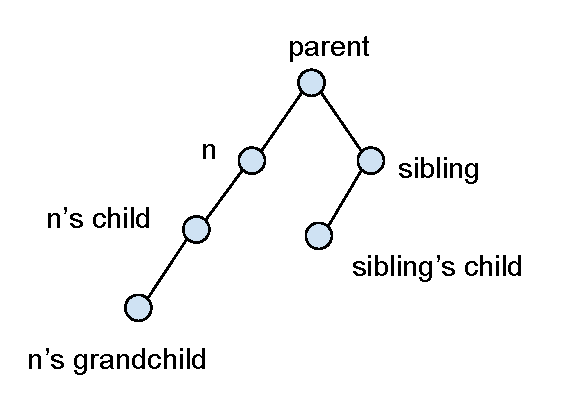
\includegraphics[width=0.7\textwidth]{P5.pdf}
    \caption{BST Walk}
    \label{fig:bst-walk}
\end{figure}
First, assume the costliest edge in the optimal Hamiltonian cycle ($H^*$) is $w^*$. Since the Halmitonian cycle is constructed by adding an edge to the BST, the costliest edge in the BST cannot exceed $w^*$. Because if the extra edge added into the BST is no heavier than $w^*$, the BST has the same cost as the cycle. Otherwise if the extra edge is heavier than $w^*$, the cycle has more cost than the BST. \\
Thus, in G, we have $c_{max}(BST^*) \leq c_{max}(H^*) = w^*$. \\

And we look at a traversal of the BST to create an HC. Assume the traversal does not skip more than two consecutive vertices in the BST, which we will describe how to later. By this property, we can derive an upper bound. In the worst case, a path can be at most distance of 3 by skipping two vertices. If all the 3 segments of that path are of costliest edges, the path weight will be $3w^*$ at most. And the HC generated from the walk will have a costliest edge of $3w^*$ at most by triangle inequality. In other words, we have a walk that $c_{max}(W) \leq 3*c_{max}(H^*)$, which means the approximation ratio is 3. \\

To implement such a walk, we define:
\begin{verbatim}
function nextNode(n):
if n is unmarked:
    mark n
    nextNode(n)
else if n has unmarked children:
    c = first unmarked child of n
    if c has unmarked children:
        x = first unmarked child of c
        nextNode(x)
    else
        nextNode(c)
else if n has unmarked siblings:
    s = first unmarked sibling of n
    p = n's parent
    if s has unmarked children and p is marked:
        y = first unmarked child of s
        nextNode(y)
    else
        nextNode(s)
else if n has a parent:
    p = n's parent
    nextNode(p)
else
    return
\end{verbatim}
We start by choosing an arbitary vertex to be root of the BST. Then call nextNode() and get a list of returned marked vertices. It would be the approximated HC. This function allows us to mark the vertices without skipping more than 2 vertices because it never goes beyond 2 levels (a level is a set of vertices sharing the same depth) of a tree. In the worst case that the 2 vertices of 2 levels are both marked previously, it still only skips 2 vertices at most. As figure \ref{fig:bst-walk} shows, for any node n, it is only aware of and reachable to its parent, its child, its grandchild, its sibling and its sibling's child. And the furthest it can reach is the child of its sibling, which is still within a distance of 3. \\

Now consider the time complexity, from problem 23-3, we can compute the BST by removing edges starting from the costliest in linear time. Taking a full walk can also easily be done in polynomial time. So overall, this algorithm is polynomial. \\




\end{document}
